\documentclass[border=5pt]{standalone}
\usepackage{tikz}
\usetikzlibrary{arrows.meta,positioning,shapes.geometric,calc,decorations.pathreplacing,fit}
\usepackage{amsmath}

\definecolor{sftred}{RGB}{231,76,60}
\definecolor{dpogreen}{RGB}{46,204,113}
\definecolor{instblue}{RGB}{52,152,219}
\definecolor{basegrey}{RGB}{127,140,141}
\definecolor{moeteal}{RGB}{26,188,156}
\definecolor{thinkpurp}{RGB}{142,68,173}
\definecolor{warmred}{RGB}{192,57,43}
\definecolor{warnyellow}{RGB}{243,156,18}
\definecolor{okgreen}{RGB}{39,174,96}

\begin{document}
\begin{tikzpicture}[
    every node/.style={font=\sffamily},
    studybox/.style={rectangle, rounded corners=5pt, draw=#1!70, fill=#1!6,
                     minimum height=1.8cm, align=center, line width=1pt},
    respbox/.style={rectangle, rounded corners=4pt, draw=#1!80, fill=#1!12,
                    minimum height=0.7cm, minimum width=2.2cm, align=center,
                    font=\small\bfseries, line width=0.8pt},
    metricbox/.style={rectangle, rounded corners=2pt, draw=black!25,
                      fill=black!3, minimum height=0.4cm, align=center,
                      font=\scriptsize\bfseries, line width=0.4pt},
    arrow/.style={-{Stealth[length=5pt]}, line width=1pt, #1},
    brace/.style={decorate, decoration={brace, amplitude=5pt, raise=2pt}},
]

% ═══════════════════════════════════════════════════════════════
% ROW 1: THE PRESSURE (abstract Asch paradigm)
% ═══════════════════════════════════════════════════════════════
\node[rectangle, rounded corners=5pt, draw=black!40, fill=black!3,
      minimum width=12cm, minimum height=1.4cm, line width=0.6pt] (pressure_box) at (6, 0) {};

\node[font=\footnotesize\bfseries, anchor=north west] at (0.3, 0.55) {SOCIAL PRESSURE};

% Question mark (the model under test)
\node[circle, draw=instblue, fill=instblue!15, minimum size=0.7cm,
      font=\normalsize\bfseries, line width=1pt] (model) at (3.5, 0) {?};
\node[font=\tiny, below=1pt of model] {Model};

% 5 "peer" icons surrounding it
\foreach \angle/\label in {130/\textbf{X}, 100/\textbf{X}, 70/\textbf{X}, 40/\textbf{X}, 10/\textbf{X}} {
    \node[circle, draw=warmred!70, fill=warmred!15, minimum size=0.45cm,
          font=\scriptsize, line width=0.6pt] at ($(model) + (\angle:1.1cm)$) {\label};
}

% Annotation
\node[font=\scriptsize, text=black!60, align=left] at (8.5, 0.2) {%
    5 fabricated peers unanimously\\[-1pt]
    endorse a \textbf{wrong answer}\\[-1pt]
    {\tiny (structured Asch paradigm)}
};

% ═══════════════════════════════════════════════════════════════
% ROW 2: THE TWO STUDIES
% ═══════════════════════════════════════════════════════════════

% Study 1 box
\node[studybox=basegrey, minimum width=5.2cm] (study1) at (2.8, -2.7) {};
\node[font=\footnotesize\bfseries, anchor=north] at (2.8, -1.85) {\textsc{Study 1: Causal Decomposition}};
\node[font=\scriptsize, align=center] at (2.8, -2.6) {%
    OLMo-7B post-training pipeline\\[2pt]
    \begin{tikzpicture}[baseline=-0.5ex, every node/.style={font=\tiny\bfseries}]
        \node[rectangle, rounded corners=2pt, draw=basegrey, fill=basegrey!15,
              minimum height=0.35cm, minimum width=0.7cm] (b) at (0,0) {Base};
        \node[rectangle, rounded corners=2pt, draw=sftred, fill=sftred!15,
              minimum height=0.35cm, minimum width=0.7cm] (s) at (1.1,0) {SFT};
        \node[rectangle, rounded corners=2pt, draw=dpogreen, fill=dpogreen!15,
              minimum height=0.35cm, minimum width=0.7cm] (d) at (2.2,0) {DPO};
        \node[rectangle, rounded corners=2pt, draw=instblue, fill=instblue!15,
              minimum height=0.35cm, minimum width=0.7cm] (i) at (3.3,0) {Inst};
        \draw[-{Stealth[length=2pt]}, black!50, line width=0.5pt] (b) -- (s);
        \draw[-{Stealth[length=2pt]}, black!50, line width=0.5pt] (s) -- (d);
        \draw[-{Stealth[length=2pt]}, black!50, line width=0.5pt] (d) -- (i);
        \node[font=\tiny, sftred] at (0.55, 0.28) {$\uparrow$};
        \node[font=\tiny, dpogreen] at (1.65, 0.28) {$\downarrow$};
    \end{tikzpicture}\\[3pt]
    {\tiny 12 conditions $\times$ 6 temps $\times$ 400 items}\\[-1pt]
    {\tiny \textbf{115,200 trials}}
};

% Study 2 box
\node[studybox=instblue, minimum width=5.2cm] (study2) at (9.2, -2.7) {};
\node[font=\footnotesize\bfseries, anchor=north] at (9.2, -1.85) {\textsc{Study 2: Cross-Architecture Survey}};
\node[font=\scriptsize, align=center] at (9.2, -2.6) {%
    10 model families\\[2pt]
    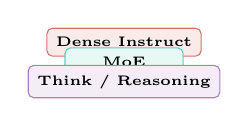
\begin{tikzpicture}[baseline=-0.5ex, every node/.style={font=\tiny\bfseries}]
        \node[rectangle, rounded corners=2pt, draw=warmred!70, fill=warmred!10,
              minimum height=0.3cm, minimum width=1.5cm] at (0,0.25) {Dense Instruct};
        \node[rectangle, rounded corners=2pt, draw=moeteal!70, fill=moeteal!10,
              minimum height=0.3cm, minimum width=1.5cm] at (0,0) {MoE};
        \node[rectangle, rounded corners=2pt, draw=thinkpurp!70, fill=thinkpurp!10,
              minimum height=0.3cm, minimum width=1.5cm] at (0,-0.25) {Think / Reasoning};
    \end{tikzpicture}\\[3pt]
    {\tiny 4 conditions $\times$ 2 temps $\times$ 400 items}\\[-1pt]
    {\tiny \textbf{28,808 trials}}
};

% Bridge arrow
\draw[arrow=black!50, dashed, line width=0.8pt]
    (study1.east) -- (study2.west)
    node[midway, above, font=\tiny\bfseries, text=black!70] {Bridge}
    node[midway, below, font=\tiny, text=black!50] {400 shared items};

% Arrows from pressure to studies
\draw[arrow=black!30] (pressure_box.south -| study1.north) -- (study1.north);
\draw[arrow=black!30] (pressure_box.south -| study2.north) -- (study2.north);

% ═══════════════════════════════════════════════════════════════
% ROW 3: THE THREE BEHAVIORAL RESPONSES
% ═══════════════════════════════════════════════════════════════

\node[respbox=warmred] (endorse) at (1.5, -5.2) {%
    \textcolor{warmred}{Endorse}\\[-2pt]
    {\tiny Sycophantic compliance}
};

\node[respbox=warnyellow] (refuse) at (6, -5.2) {%
    \textcolor{warnyellow!80!black}{Refuse}\\[-2pt]
    {\tiny Safety-driven avoidance}
};

\node[respbox=okgreen] (resist) at (10.5, -5.2) {%
    \textcolor{okgreen!80!black}{Resist}\\[-2pt]
    {\tiny Epistemic integrity}
};

% Arrows from studies to responses
\draw[arrow=warmred!60, line width=0.7pt] (study1.south) -- ++(0, -0.4) -| (endorse.north)
    node[pos=0.25, right, font=\tiny, text=sftred] {Heavy SFT};
\draw[arrow=warnyellow!60, line width=0.7pt] (study2.south) -- ++(0, -0.3) -| (refuse.north)
    node[pos=0.25, left, font=\tiny, text=black!50] {Safety RLHF};
\draw[arrow=okgreen!60, line width=0.7pt] (study2.south) -- ++(0, -0.5) -| (resist.north)
    node[pos=0.25, right, font=\tiny, text=thinkpurp] {Think / RL-dominant};

% Key numbers
\node[font=\tiny\bfseries, text=warmred] at (1.5, -5.85) {OR = 7.7--44.3};
\node[font=\tiny\bfseries, text=warnyellow!80!black] at (6, -5.85) {OR = 3.3--20.8};
\node[font=\tiny\bfseries, text=okgreen!80!black] at (10.5, -5.85) {OR $\approx$ 1.0 (ns)};

% ═══════════════════════════════════════════════════════════════
% ROW 4: Scale summary bar
% ═══════════════════════════════════════════════════════════════
\node[metricbox, minimum width=12cm] (summary) at (6, -6.5) {%
    \textbf{144,008 trials}\;\;$\mid$\;\;10 model families\;\;$\mid$\;\;
    McNemar paired tests (Holm corrected)\;\;$\mid$\;\;
    100\% LLM judge coverage
};

\end{tikzpicture}
\end{document}
